\documentclass[portfolio.tex]{subfiles}
\begin{document}
	\Chapter{Week 4}{TCP/IP}


		\section{Weekly Content}
				\subsection{Introduction}
					The theoretical portion of this weeks information was based around the TCP/IP Protocol. This is how most computers communicate across the internet. It is important to understand not only design principles, and programming languages in web development, but also how the internet itself works.\\

			\subsection{TCP/IP Protocol}
				\subsection{Data packets}
					Files are too large to send all at once over the internet. Instead we break them up into many packets, and send them one at a time. The size of these packets may vary, but the point is that there are many of them for one file.\\

				\subsection{Application Layer}
					This layer is specific to each type of application and is how the applications connect to the internet. Each type of application will be given a port number. This allows many different services/applications to be running on a particular computer at one time. This also creates standards, so applications of the same type can communicate with each other effectively. An example of this is HTTP. This tells browsers and web servers how to communicate with each other. All of this information is bundled as a header on the data packet, and passed to the TCP layer. \autocite{stanford-internet}

				\subsubsection{TCP}
					If the application layer is how applications communicate, then the TCP layer is how computers communicate. This is a set of standard pieces of information put together in a very specific format. This includes information like the number of packets being sent, a checksum to ensure no corruption, etc.

				\subsubsection{IP}
					\label{ip} Now that we have all the information, the next part to be applied is the IP address or \textbf{WHERE} to send the packet. This is unique for each computer in the world, and is bundled on top of the tcp layer.

				\subsubsection{Data-link}
					\label{mac}
					Finally the data-link layer is associated with the physical machines themselves. This is how the short jumps are addressed, from router to router as the message travels to its destination.

				\begin{center}
					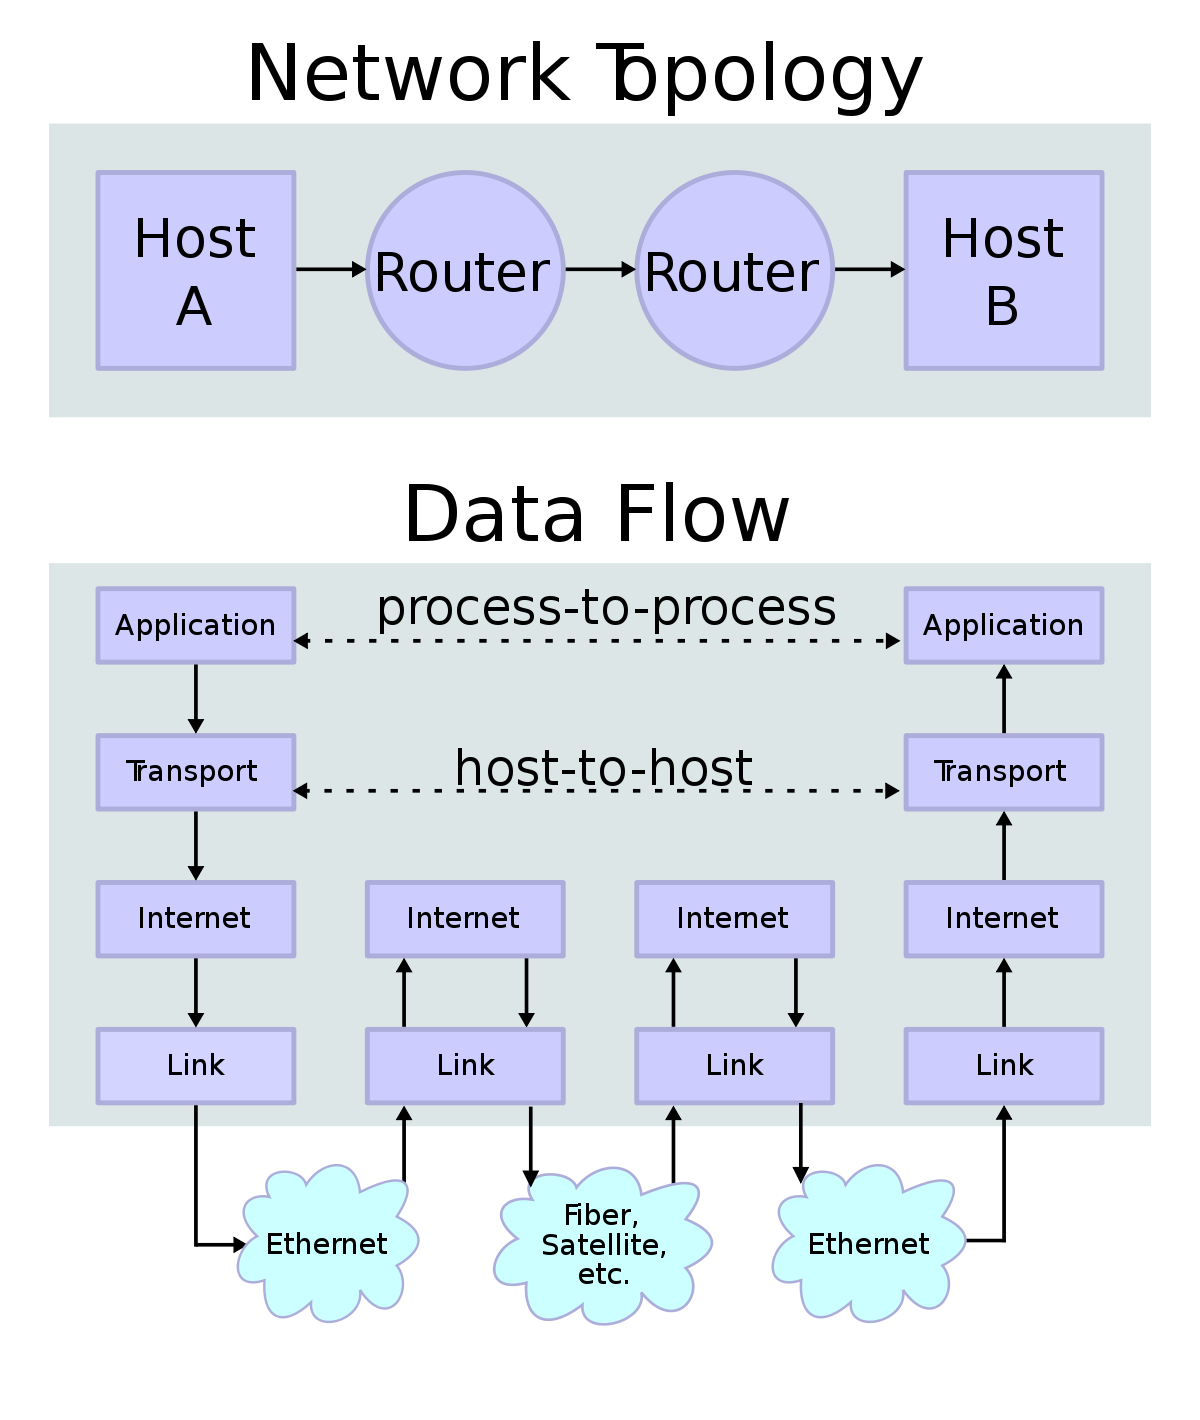
\includegraphics[width=0.6\textwidth]{IP-stack.png}\\
					\autocite{network-topology}
				\end{center}

			\subsection{Routing}
				\subsubsection{DNS}
					DNS or Domain Name System is an electronic address book for websites. Instead of having to remember the IP addresses of the web server you would like to visit, it allows users to remember more human-friendly addresses, such as www.deakin.edu.au. \autocite{stanford-internet} This is similar to a phone book, where instead of remembering the phone number, you only have to remember the persons name. \\

					Each time before connecting to a server, your computer must first get the IP address from the DNS server, so that it knows where to send the data.
				\subsubsection{Pathway}
					The internet isn't one solid "thing". Instead it is made up of many computers/routers/etc. To be able to communicate with another specific computer, the message must pass through a chain of many other routers. This uses the MAC address discussed in \ref{mac} and the IP address discussed in \ref{ip}. \\

					Starting from the source computer, each computer finds a router which is closer to the end destination. The message is then sent to a router that is closer to the destination ip address using the router's mac address. Then that router finds a closer router and passes the message along. This continues until the message finally gets to the destination.

					But what are these routers? Surely they aren't just the same routers in your home... No, these are large industrial routers, and usually the first hop will be to your ISP (Internet Service Provider), then a second one will be to a larger router(or groups of routers) called an NSP (Network Service Provider). From here they can connect to other NSPs via an NAP (Network access Point) or MAE (Metropolitan Area Exhanges).   \autocite[The Internet Routing Hierarchy]{stanford-internet}\\

					\hspace{-0.9cm}
					\splitpage{
						The beauty of this is two fold. First of all, there is no "set path" that a message must travel. This helps to relieve congestion within the network. Secondly, if there is a break in the chain, it is very easy for the routers to reroute the message to another router, as long as it is closer to the destination.
					}{
						\centering
						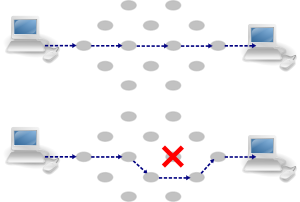
\includegraphics[width=0.9\textwidth]{internet-routing.png}
						\autocite{routing-reroute}
					}
		\section{Practical Tasks}

			\subsection{Introduction}
				The practical tasks this week all focused on beginning to create websites in Vue. Using concepts that we researched last week such as declarative rendering,  and conditionals, we are again able to reduce the amount of code needed compared to writing in plain HTML/CSS/JavaScript.

			\subsection{Task 1}
				Declarative rendering in Vue is about dynamically creating webpages based on templates. In the templates, placeholders will use double curly brackets \{\{\}\},with the placeholder name being inside. This placeholder name will map to a variable in the Vue/Javascript code. During rendering, Vue will grab the variable value and place it in the placeholder. This way, each time the user visits the webpage, it can present different information based on their query without writing millions of possible HTML pages.\\

				This becomes even more powerful, when different images, links, etc can be loaded into the template. So that the same page layout can look drastically different. \\

				For evidence of the completion of this tasks, I will provide the work in Vue I did for my proof of concept. I used declarative rendering throughout the application. Here is one example where the same coloured boxes are the same parts of a template. They are just filled with different data:\\

				\begin{center}
					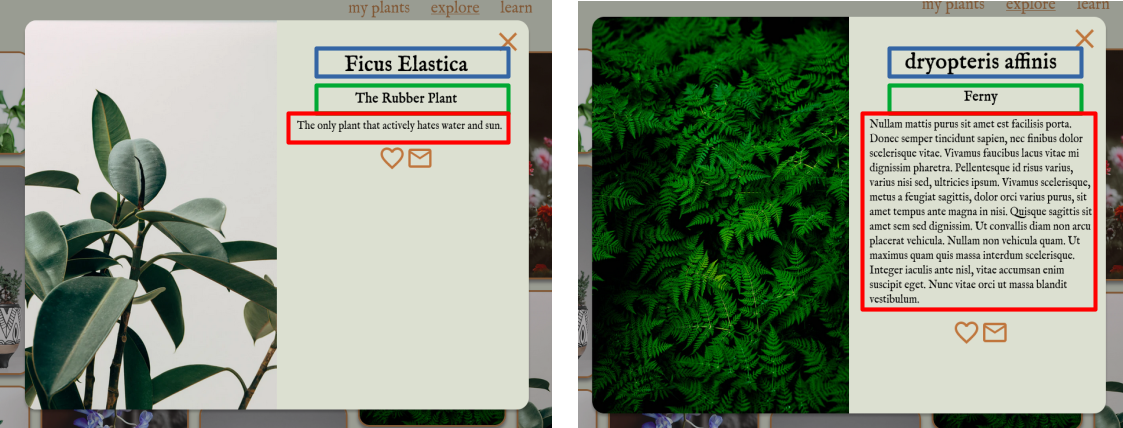
\includegraphics[width=0.8\textwidth]{template-use.png}
				\end{center}



				See examples of my proof of concept at \seqsplit{https://github.com/BrandonMurch/SIT120/tree/main/Assignment\%201/proof-of-concept} \\

				The specific example is found at \seqsplit{https://github.com/BrandonMurch/SIT120/blob/021a2694432d61e32c9fba191ee7579c2dfdb955/Assignment\%201/proof-of-concept/src/components/PopUp.vue}

			\subsection{Task 2}
				Conditionals are a way of selecting whether to display a component or not. If the particular variable is true, the component will be rendered. If not, the component will not be rendered at all. The syntax for this within Vue is v-if, v-else, v-else-if. Within my project I used this for a few things. Firstly, I used it in my main profile page as a mock router to switch between pages before I implement Vue-Router. I also used it to render the pop up if a plant was selected. If there was no plant selected, the pop up would not appear. Finally, a very visual example is using v-if to toggle when the pop-up is displayed. If a plant is stored in "popUpImage" then the pop up will be displayed, otherwise it won't. \\

				\hspace{-0.8cm}
				\splitpage{
					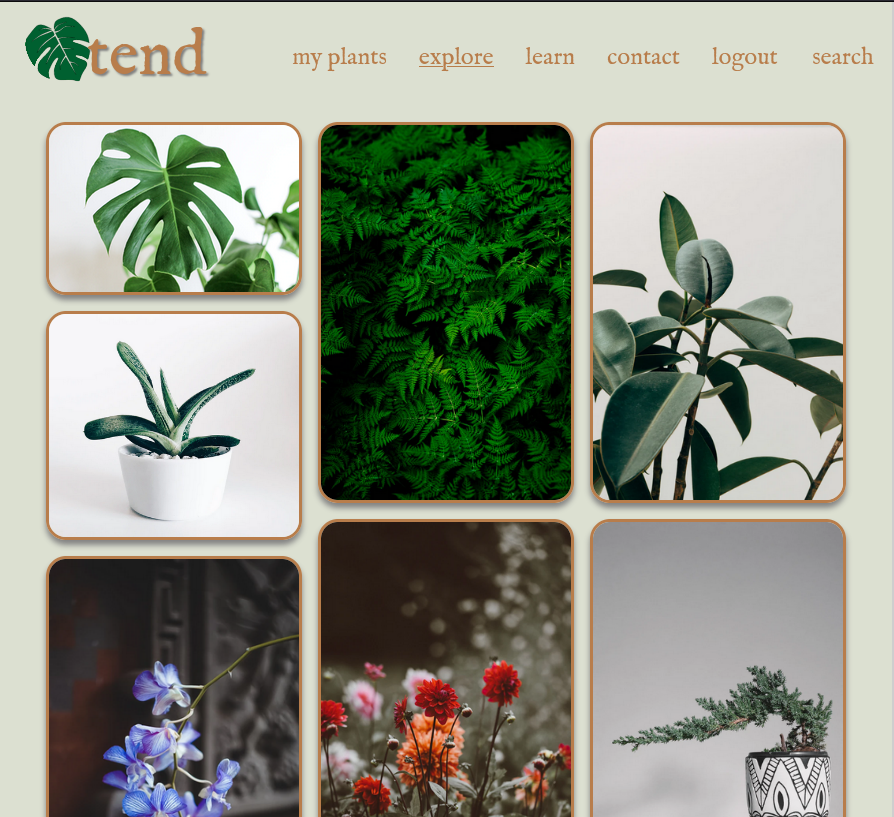
\includegraphics[width=0.9\textwidth]{no-pop-up.png}
				}{
					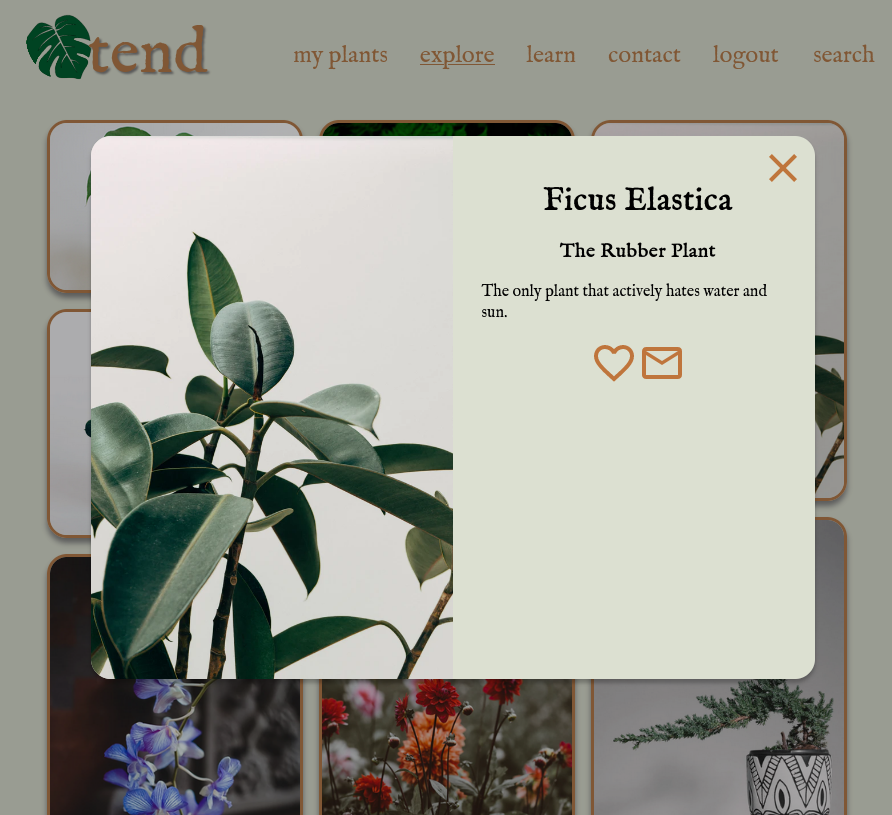
\includegraphics[width=0.9\textwidth]{with-pop-up.png}
				}\\

				\bigbreak
				There is an alternative syntax of v-show which still renders the component (unlike v-if), but hides it using CSS.\\

				Loops are used for rendering multiple elements, with a single template element. I used this frequently to reduce the amount of code. For example, instead of creating each navigation link, I created a template, then looped over an array to insert information for each link. The example below shows that each blue box is actually the same element, but using v-for to create multiple.\\

				\begin{center}
					
\includegraphics[width=0.7\textwidth]{v-for-nav.png}
				\end{center}

				\subsubsection{Source Code}

				\noindent See examples of my proof of concept at \seqsplit{https://github.com/BrandonMurch/SIT120/tree/main/Assignment\%201/proof-of-concept}\\

				\noindent The specific example for v-if is located at \seqsplit{https://github.com/BrandonMurch/SIT120/blob/021a2694432d61e32c9fba191ee7579c2dfdb955/Assignment\%201/proof-of-concept/src/components/ImageGallery.vue}\\

				\noindent The specific example for v-for is located at \seqsplit{https://github.com/BrandonMurch/SIT120/blob/021a2694432d61e32c9fba191ee7579c2dfdb955/Assignment\%201/proof-of-concept/src/components/NavigationLinks.vue}
		\section{Project}
			\subsection{What I accomplished this week}

				I focused on my proof of concept this week. I was able to complete the explore portion of my application. Within this section I was also able to create the following components: ImageGallery, SearchBar, ImageCard, NavigationBar, ContactForm, PopUp, and MenuIcon. \\

				While doing this, I also explored several more advanced topics within Vue.\\

				\subsubsection{Custom Events}
					\label{custom-events}
					Within Vue there are ways to create custom events. These react the same way as native HTML events, such as @click or v-on:click.\\

					To create a custom event within the child component, Vue allows the use of the emit method, with the following syntax: this.\textbf{\$emit('customEvent')}. This will send the custom event to the parent component whenever it is called. To let the parent know that the child is capable of emitting this custom event, it must be placed in the \textbf{emits }array like so:\\

					\begin{lstlisting}
<script>
	export default {
		...
		emits: ["customEvent"],
		...
	}
</script>
					\end{lstlisting}


					To react to the event in the parent component, simply use the same syntax as native events. Continuing the example of 'customEvent', the syntax used is \textbf{@customEvent="..."}.\\

					A second argument can be passed into \$emit to pass a variable through to the parent component. This allows the ability for two way binding, where two variables can be linked in both the parent and child. Changing the value in one, will change the value in the other. The syntax for this would be:\\ \textbf{@customEvent="(data) => variable = data"}\autocite{vue-custom-event}


					\splitpage{
						\subsubsection{Vue Component Lifecycle}
						Vue allows functions to be called at certain points relative to the creation of a component. Some options are:

						\begin{itemize}
							\item create - Data, properties, etc. are available, but the element has not been rendered.
							\item mounted - Element has been rendered in the DOM for the first time.
							\item updated - A data change has caused the component to update.
							\item unmounted - The component has been destroyed, removing it from the DOM, and memory.
						\end{itemize}

						More hooks can be found here: \autocite{vue-lifecycle}.
					}{
						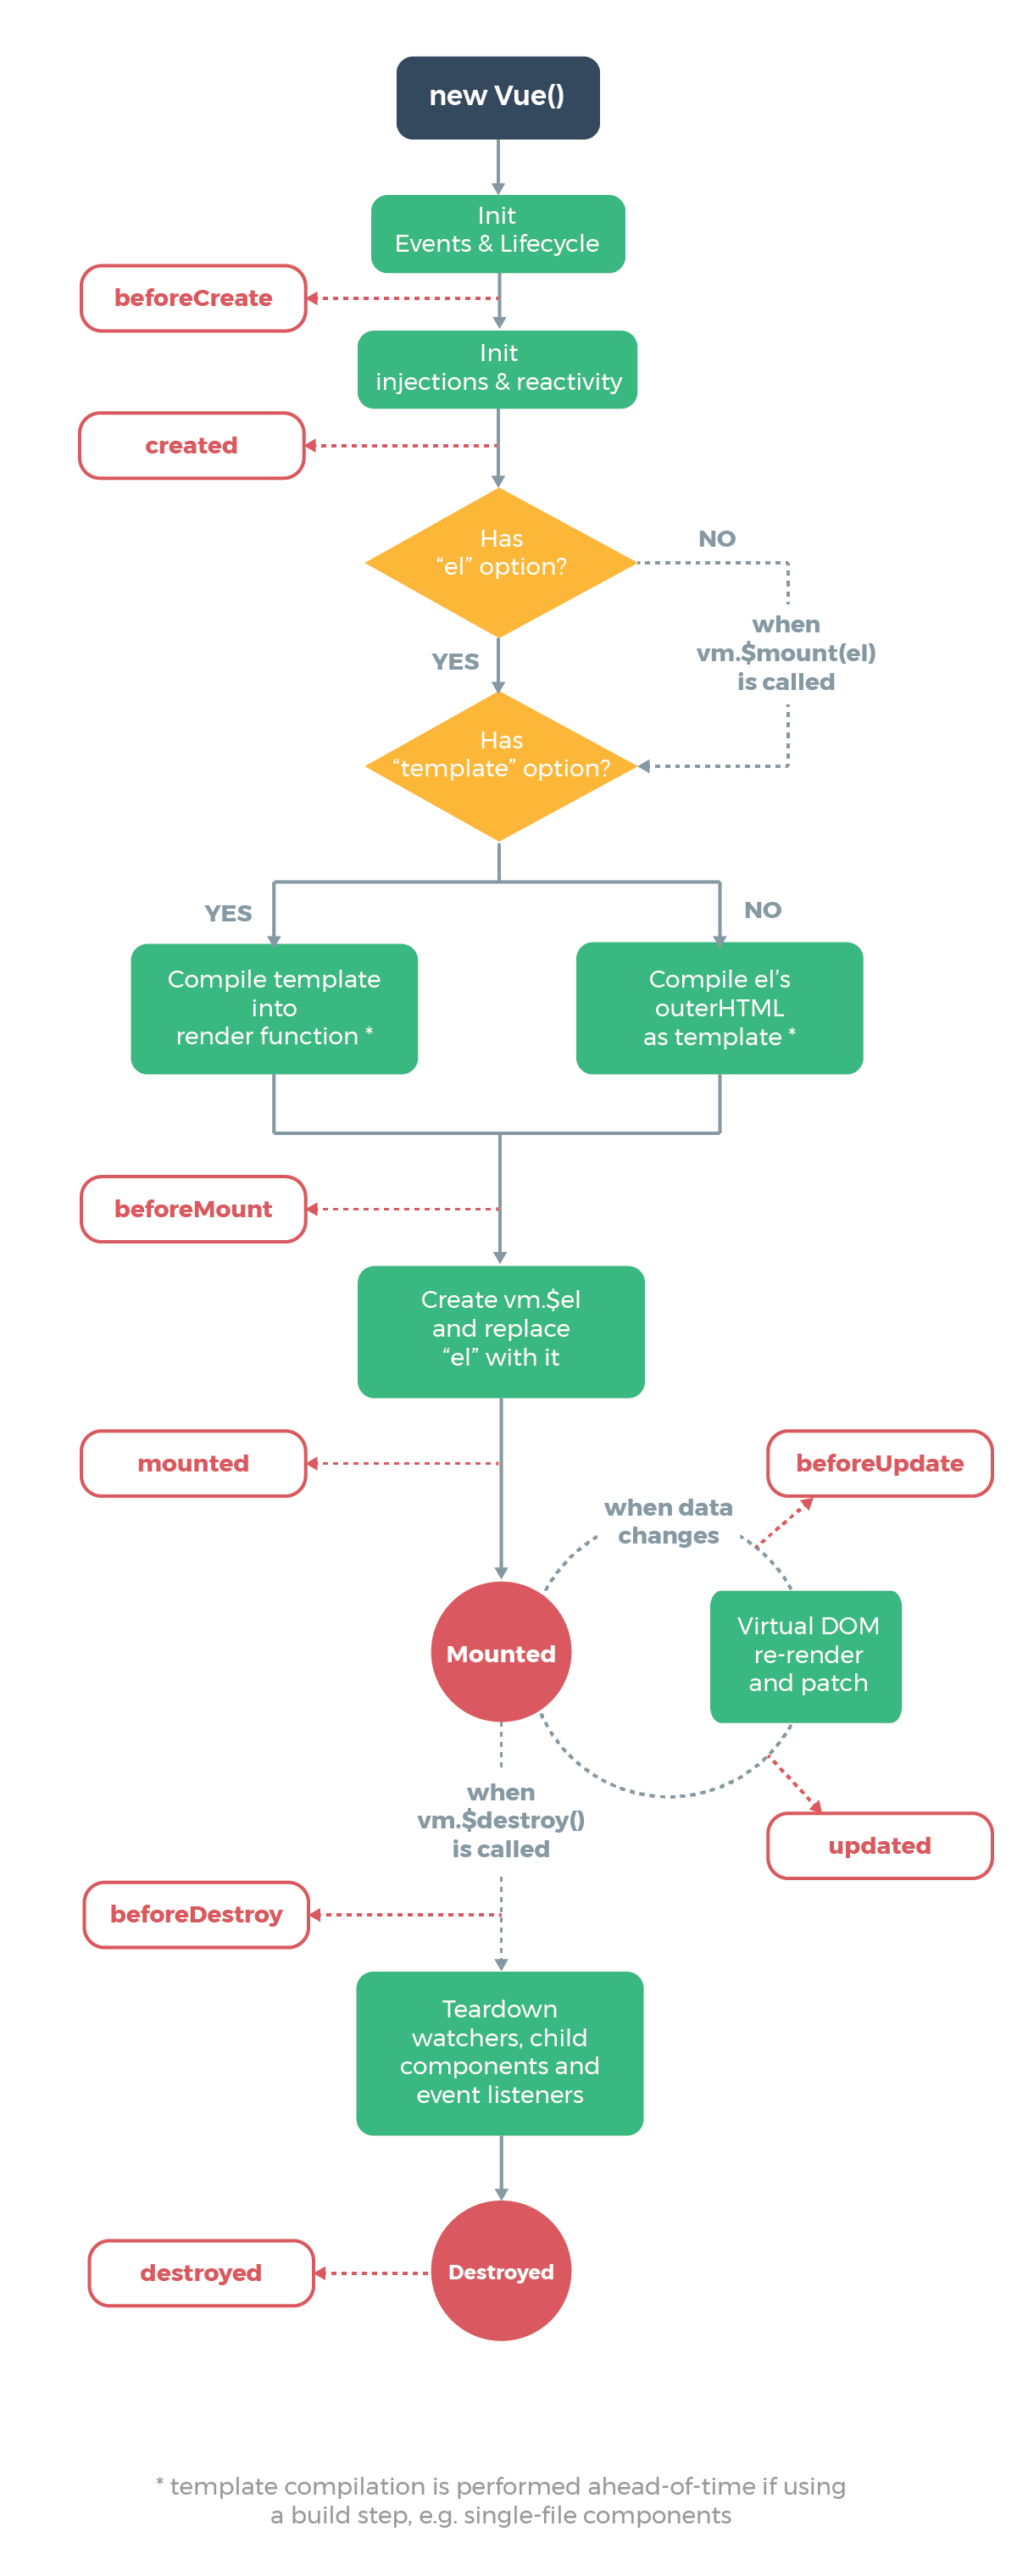
\includegraphics[width=0.9\textwidth]{vue-lifecycle.png}
					}

				\subsubsection{Slots}
					\label{slots}
					Slots are a way for full components or html to be easily passed into another component. In addition to the default slot, slots can be named for multiple slots in one component. \\

					To define the slot space, the slot element is used. To name it, use the name attribute. For example: \textbf{$<$slot name="slotName" /$>$}.\\

					In the parent component, a default slot can be used like any HTML tag. Simply put the slot template inside the child like so:\\

					\begin{lstlisting}
<template>
	<ChildComponent>
		<h1> This will go inside the child! </h1>
	</ChildComponent>
</template>
					\end{lstlisting}

					\bigbreak
					The template element is used to define what should be put inside a named slot. To choose which named slot to use, the v-slot:name attribute is used. So to place html in the previously mentioned slot, the syntax would be:\\

					\begin{lstlisting}
<template>
	<ChildComponent>
		<template v-slot:title>
			<h1> This will go inside the child in the "title" slot!</h1>
		</template>
	</ChildComponent>
</template>
					\end{lstlisting}



				\subsubsection{Refs}
					Refs give developers a way to reference components without having to use id or class. This is done by first setting the ref attribute on the component using a string. For example:
					\begin{center}
						\textbf{<component ref="referenceString" />}\\
					\end{center}


					\noindent Then the component can be grabbed by using:

					\begin{center}
						 \textbf{this.\$ref.referenceString}\\
					\end{center}


					\noindent \autocite{vue-refs}

				\subsubsection{Unrelated to Vue}
					Unrelated to Vue, I also looked into the following:
					\begin{itemize}
						\item CSS Transitions (\ref{css-transitions})
						\item Modifying the scrollbar with CSS (\ref{css-scrollbar})
						\item "Debounce" (\ref{js-debounce})
						\item Array Filter (\ref{css-scrollbar})
					\end{itemize}

			\subsection{What I would like to accomplish next week}
				This week I would like to incorporate Vue-Router into my program, and start creating the other parts of the website (My Plants, and Learn). The main reusable components I will need for this are lists to display cards for comments, articles, etc. Another important part will be to create the interface for adjusting plant settings. I suspect this all will take 4 hours.

\pagebreak
\end{document}